\documentclass{beamer}

\usepackage{preamble}

\begin{document}

\begin{frame}
    \titlepage
\end{frame}

\begin{frame}{Outline}
    \tableofcontents
\end{frame}

\tikzset{g/.style={
            prefix after command= {\pgfextra{\tikzset{every label/.style={color=green,above left}}}}
}
}

\tikzset{r/.style={
            prefix after command= {\pgfextra{\tikzset{every label/.style={red,above left}}}}
}
}

\tikzset{o/.style={
            prefix after command= {\pgfextra{\tikzset{every label/.style={orange,above left}}}}
}
}

\section{Examples}

\begin{frame}{Example: Blacklist}
    Property: no packets from $a$ should reach $d$
    \begin{center}
        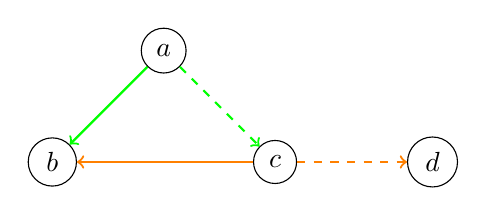
\begin{tikzpicture}[
                node distance={20mm},
                main/.style = {draw, circle},
                s/.style = {->,thick},
                d/.style = {->,thick,dashed} ]
            \node[main] (b) {$b$};
            \node[main] (a) [above right of=b] {$a$};
            \node[main] (c) [below right of=a] {$c$};
            \node[main] (d) [right of=c] {$d$};
            \draw[thick,green,->] (a) -- (b);
            \draw[thick,green,->,dashed] (a) -- (c);
            \draw[thick,orange,->] (c) -- (b);
            \draw[thick,orange,->,dashed] (c) -- (d);
        \end{tikzpicture}
    \end{center}
    \begin{equation*}
        \begin{aligned}[c]
            P   & = p!1                             \\
            Q   & = q!1                             \\
            N   & = F \oplus p?1;N_p \oplus q?1;N_q \\
            N_p & = F_p \oplus q?1;F_{pq}           \\
            N_q & = F_q \oplus p?1;F_{pq}           \\
            F   & = ab \oplus cb                    \\
        \end{aligned}
        \qquad\qquad
        \begin{aligned}[c]
            F_p         & = ac \oplus cb \oplus ab  \\
            F_q         & = ab \oplus cd            \\
            F_{pq}      & = ac \oplus cd \oplus ad  \\
            SDN         & = \delta_{\mathcal{L}} (N
            \parallel P \parallel Q)                \\
            \mathcal{L} & = \s{p!1,p?1,q?1,q?1}     \\
        \end{aligned}
    \end{equation*}
\end{frame}

\begin{frame}{Example: Blacklist}
    Property: no packets from $a$ should reach $d$
    \begin{align*}
        \f{PV} & = \bigvee_{c \in C} c \in \mathcal{F}(ES(\vec v))       \\
        C      & = \s{c \subseteq E | \exists e \in c. l(c) = ad } 
    \end{align*}
    We can define $C(p_1,q_1) = \F$ as an actual cause of $PV$
    using the witness $(C(p_2,q_2),\T,\T)$
    \begin{center}
        \begin{tikzpicture}[scale=0.8]
            \crd{0}{0}{$\emptyset$}
            \crd[left]{-2}{1}{$\s{p_1}$}
            \crd[left]{-2}{2}{$\s{p_1,q_1}$}
            \crd[left]{-2}{3}{$\s{p_1,q_1,ad_1}$}
            \crd[right]{2}{1}{$\s{q_2}$}
            \crd[right]{2}{2}{$\s{p_2,q_2}$}
            \crd[right]{2}{3}{$\s{p_2,q_2,ad_2}$}
            \draw [ultra thick] (-2,1) -- (-2,2);
            \draw [ultra thick] (-2,2) -- (-2,3);
            \draw [ultra thick] (0,0) -- (2,1);
            \draw [ultra thick] (0,0) -- (-2,1);
            \draw [ultra thick] (2,1) -- (2,2);
            \draw [ultra thick] (2,1) -- (2,3);
        \end{tikzpicture}
    \end{center}
\end{frame}

\begin{example}
    \begin{figure}
        \centering
        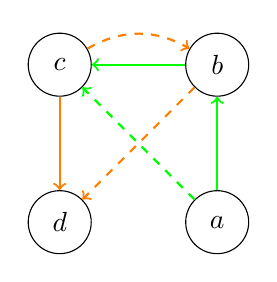
\begin{tikzpicture}[node distance={20mm},main/.style = {draw, circle,minimum size=8mm}]
            \node[main] (a)  {$a$};
            \node[main] (b) [above of=a]  {$b$};
            \node[main] (c) [left of=b] {$c$};
            \node[main] (d)  [below of=c] {$d$};
            \draw [->,green,thick] (a) -- (b);
            \draw [->,green,thick] (b) -- (c);
            \draw [->,orange,thick] (c) -- (d);
            \draw [->,green,thick,dashed] (a) -- (c);
            \draw [->,orange,thick,dashed] (c) edge[bend left] (b);
            \draw [->,orange,thick,dashed] (b) -- (d);
        \end{tikzpicture}
        \caption{ }
        \label{fig:loop}
    \end{figure}
    Loop-freedom property requires the network to not contain loop
    at any given moment \cite{network-abstractions}.
    For example consider the network in figure \ref{fig:loop}.
    Initially, there exists a path from $a$ to $d$.
    Assume that we wish to update this route to first visit $c$.
    Here we assume that two updates make this transition, one
    replacing green solid path with the dashed and the other
    replacing the orange solid path with the dashed path.
    We can encode this network as the following DyNetKAT terms:
    \begin{equation*}
        \begin{aligned}
            P           & = p!1                                             \\
            Q           & = q!1                                             \\
            N           & = F \oplus p?1;N_p \oplus q?1;N_q                 \\
            N_p         & = F_p \oplus q?1;F                                \\
            N_q         & = F_q \oplus p?1;F                                \\
            SDN         & = \delta_{\mathcal{L}}(N \parallel P \parallel Q) \\
            \mathcal{L} & = \s{p!1,p?1,q!1,q?1}
        \end{aligned}
        \qquad \qquad
        \begin{aligned}
            F    = & a\ra b \oplus a\ra c \oplus a\ra d               \\
                   & \oplus b\ra c \oplus b\ra d \oplus c\ra d        \\
            F_p  = & a\ra c \oplus a\ra d \oplus c\ra d               \\
            F_q  = & a\ra b \oplus a\ra c \oplus a\ra d               \\
                   & \oplus b\ra c \oplus b\ra b \oplus b\ra d        \\
                   & \oplus        c\ra b \oplus c\ra c \oplus c\ra d
        \end{aligned}
    \end{equation*}
    Here we assume two concurrent processes for $P$ and $Q$ for updating
    the green and orange paths respectively.
    It is obvious that in this network if $rcfg(q,1)$ happens while
    $rcfg(p,1)$ has not happened yet, then a loop including
    $b$ and $c$ would be created.
    Let $\mr{E} = \sem{SDN}$ an $\mc{M}$ be the causal model of $\mr{E}$.
    Here we can define the unsafe in an event structure as existence of
    a configuration that includes an event with label of the form
    $\alpha\cdot\pi$ where $\alpha(sw) = \pi(sw)$.
    So, we can encode the function of $PV$ as follows:
    \begin{align*}
        \f{PV} = \exists c \in \mc{F}(ES(\vec v)).
        l(c) = \alpha\cdot\pi \Rightarrow \alpha(sw) = \pi(sw)
    \end{align*}
    This function simply checks for the existence of configuration with
    events labeled as $x \ra x$.
    We can see that in $SDN$ there are only two such actions:
    $b\ra b$ and $c\ra c$.
    Like the previous example, there are two order of execution for
    $rcfg(p,1)$ and $rcfg(q,1)$ thus we need two events to represent
    them.
    So let's consider events $p_1$ and $p_2$ with label $rcfg(p,1)$
    and events $q_1$ and $q_2$ with label $rcfg(q,1)$.
    We also consider events $bb$ and $cc$ with labels
    $b \ra b$ and $c\ra c$ respectively.
    Figure \ref{fig:loop:es} shows a part of the $\mr{E}$ where
    events $bb$ and $cc$ are reachable.
    In this model we can introduce $M(\s{p_2},q_2) = \F$ as a cause
    of loop considering $(\e,\e,\T)$ as a witness.
    In the $\mc{M}$ functions of $M_{\e,q_2}$ and $EN_{\e,q_2}$ are
    defined as follows:
    \begin{align*}
        \f{M_{\e,q_2}}  & = Min(\e,q_2) \wedge Con(\e) \\
                        & = Min(\e,q_2)                \\
                        & =  \bigwedge_{q_2 \notin s'}
        \neg M_{s',q_2}                                \\
        \f{EN_{\e,q_2}} & = M_{\e,q_2}
    \end{align*}
    Regarding the definition of these functions if we set $M_{\s{p_2},q_2}$
    to $\T$ then $M_{\e,q_2}$ and subsequently $EN_{\e,q_2}$ becomes $\F$.
    More formally we can say:
    \begin{equation*}
        M \vDash [M_{\s{p_2},q_2} \la T] M_{\e,q_2} = \F \wedge
        EN_{\e,q_2} = \F
    \end{equation*}
    Thus in $ES(\vec v)$, $\s{q_2}$ and all other configuration in the
    right branch of the figure \ref{fig:loop:es} are no longer a
    configuration which means that the property is no longer violated.
    Since we have considered and empty $\vec W$ in the witness and
    the AC2.a condition is satisfied we can conclude that $M_{\s{p_2},q_2}$
    is a cause of loop in this network.
    Intuitively $M_{\s{p_2},q_2} = \F$ means $p_2$ not happening before
    $q_2$ is an actual cause of the loop.

    \begin{figure}
        \centering
        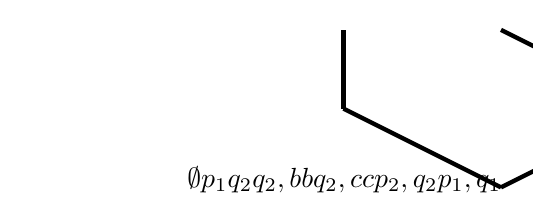
\begin{tikzpicture}
            \crd{0}{0}{$\emptyset$}
            \crd[below]{-2}{1}{$\s{p_1}$}
            \crd[below]{2}{1}{$\s{q_2}$}
            \crd[above]{2}{2}{$\s{q_2,bb}$}
            \crd[above]{4}{2}{$\s{q_2,cc}$}
            \crd[above]{0}{2}{$\s{p_2,q_2}$}
            \crd[left]{-2}{2}{$\s{p_1,q_1}$}
            \draw [ultra thick] (0,0) -- (2,1);
            \draw [ultra thick] (0,0) -- (-2,1);
            \draw [ultra thick] (2,1) -- (0,2);
            \draw [ultra thick] (2,1) -- (2,2);
            \draw [ultra thick] (2,1) -- (4,2);
            \draw [ultra thick] (-2,1) -- (-2,2);
        \end{tikzpicture}
        \caption{}
        \label{fig:loop:es}
    \end{figure}

\end{example}

\begin{frame}
    \begin{center}
        \begin{tikzpicture}[node distance={20mm},main/.style = {draw, circle,minimum size=8mm}]
            \node[main] (h1)  {$h_1$};
            \node[main] (w) [right of=h1]  {$w$};
            \node[main] (s)  [above of=h1] {$s$};
            \node[main] (h2) [right of=s2]  {$h_2$};
            \draw[->] (h1) -- node[above]{1} (w);
            \draw[->] (w) --   (h2);
            \draw[->] (s) --  node[above]{3} (h2);
        \end{tikzpicture}
        \begin{tikzpicture}[node distance={20mm},main/.style = {draw, circle,minimum size=8mm}]
            \node[main] (h1)  {$h_1$};
            \node[main] (w) [right of=h1]  {$w$};
            \node[main] (s)  [above of=h1] {$s$};
            \node[main] (h2) [right of=s2]  {$h_2$};
            \draw[->] (h1) -- node[left]{2} (s);
            \draw[->] (s) --   node[above]{4}(w);
            \draw[->] (w) --   (h2);
        \end{tikzpicture}
    \end{center}
    Property:
    \begin{itemize}
        \item Property: no forwarding loop
    \end{itemize}
    Current Behavior:
    \begin{enumerate}
        \item Replace path 1 with 2
    \end{enumerate}
\end{frame}

\begin{frame}
    \begin{center}
        \begin{tikzpicture}[node distance={20mm},main/.style = {draw, circle,minimum size=8mm}]
            \node[main] (h1)  {$h_1$};
            \node[main] (w) [right of=h1]  {$w$};
            \node[main] (s)  [above of=h1] {$s$};
            \node[main] (h2) [right of=s2]  {$h_2$};
            \draw[->] (h1) -- node[above]{1} (w);
            \draw[->,dashed] (h1) -- node[left]{2} (s);
            \draw[->] (w) --   (h2);
            \draw[->] (s) --  node[above]{3} (h2);
            \draw[->,dashed] (s) --  node[above]{4} (w);
        \end{tikzpicture}
        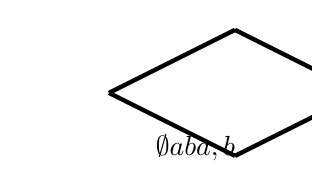
\begin{tikzpicture}[scale=0.8]
            \crd{0}{0}{$\emptyset$}
            \crd[left]{-2}{1}{$\s{a}$}
            \crd[right]{2}{1}{$\s{b}$}
            \crd[right]{0}{2}{$\s{a,b}$}
            \draw [ultra thick] (0,0) -- (2,1);
            \draw [ultra thick] (0,0) -- (-2,1);
            \draw [ultra thick] (-2,1) -- (0,2);
            \draw [ultra thick] (2,1) -- (0,2);
        \end{tikzpicture}
    \end{center}
    Events:
    \begin{itemize}
        \item $a$: Replace path 1 with 2
        \item $b$: Replace path 3 with 4
    \end{itemize}
    Counterexample: $\sigma = \s{a}$
\end{frame}


\begin{frame}{Congestion Control}
    \begin{center}
        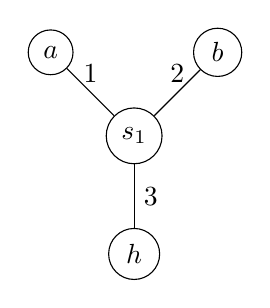
\begin{tikzpicture}[node distance={15mm},main/.style = {draw, circle}]
            \node[main] (s) {$s_1$};
            \node[main] (h) [below of=s] {$h$};
            \node[main] (a) [above left of=s]{$a$};
            \node[main] (b) [above right of=s]{$b$};
            \draw (a) --  node[above]{1}(s);
            \draw (b) --  node[above]{2}(s);
            \draw (s) --  node[right]{3}(h);
        \end{tikzpicture}
    \end{center}
    Consider a network where wish to forward traffic from $a$ and $b$ to $c$, while limiting the traffic on link 3 so that
    at any moment there must be at most one packet traversing this link.
\end{frame}

\begin{frame}
    \begin{center}
        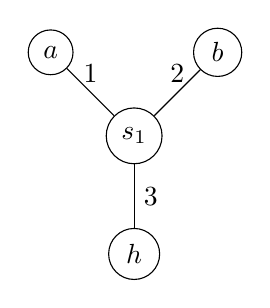
\begin{tikzpicture}[node distance={15mm},main/.style = {draw, circle}]
            \node[main] (s) {$s_1$};
            \node[main] (h) [below of=s] {$h$};
            \node[main] (a) [above left of=s]{$a$};
            \node[main] (b) [above right of=s]{$b$};
            \draw (a) --  node[above]{1}(s);
            \draw (b) --  node[above]{2}(s);
            \draw (s) --  node[right]{3}(h);
        \end{tikzpicture}
    \end{center}
    We define events $a,b$ representing the forwarding of a packet from
    1 to 3 and 2 to 3 respectively.
    We define an event $c$ when congestion is detected on link 3 (at least two packets are being traversed through the link).
    For this network, we can define an event structure $\mathrm{E}$
    with an empty conflict relation and an enabling relation the least
    one for which we have:
    \begin{align*}
        \e \vdash a, \e \vdash b, \s{a,b} \vdash c
    \end{align*}
\end{frame}

\begin{frame}
    \begin{center}
        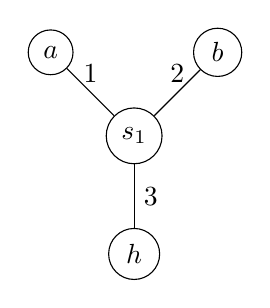
\begin{tikzpicture}[node distance={15mm},main/.style = {draw, circle}]
            \node[main] (s) {$s_1$};
            \node[main] (h) [below of=s] {$h$};
            \node[main] (a) [above left of=s]{$a$};
            \node[main] (b) [above right of=s]{$b$};
            \draw (a) --  node[above]{1}(s);
            \draw (b) --  node[above]{2}(s);
            \draw (s) --  node[right]{3}(h);
        \end{tikzpicture}
    \end{center}
    Event structure of this network has configurations of the form:
    \begin{center}
        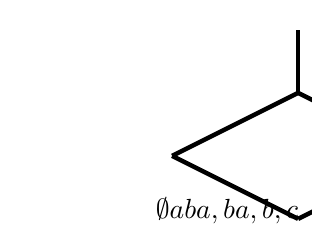
\begin{tikzpicture}[scale=0.8]
            \crd{0}{0}{$\emptyset$}
            \crd[above]{-2}{1}{$\s{a}$}
            \crd[above]{2}{1}{$\s{b}$}
            \crd[left]{0}{2}{$\s{a,b}$}
            \crd[left]{0}{3}{$\s{a,b,c}$}
            \draw [ultra thick] (0,0) -- (-2,1);
            \draw [ultra thick] (0,0) -- (2,1);
            \draw [ultra thick] (-2,1) -- (0,2);
            \draw [ultra thick] (2,1) -- (0,2);
            \draw [ultra thick] (0,2) -- (0,3);
        \end{tikzpicture}
    \end{center}
\end{frame}

\begin{frame}
    \begin{center}
        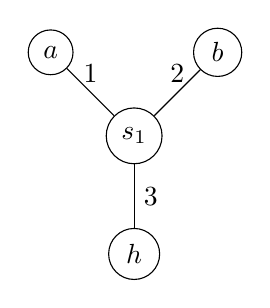
\begin{tikzpicture}[node distance={15mm},main/.style = {draw, circle}]
            \node[main] (s) {$s_1$};
            \node[main] (h) [below of=s] {$h$};
            \node[main] (a) [above left of=s]{$a$};
            \node[main] (b) [above right of=s]{$b$};
            \draw (a) --  node[above]{1}(s);
            \draw (b) --  node[above]{2}(s);
            \draw (s) --  node[right]{3}(h);
        \end{tikzpicture}
        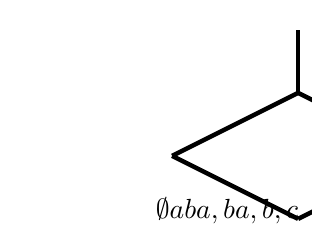
\begin{tikzpicture}[scale=0.8]
            \crd{0}{0}{$\emptyset$}
            \crd[above]{-2}{1}{$\s{a}$}
            \crd[above]{2}{1}{$\s{b}$}
            \crd[left]{0}{2}{$\s{a,b}$}
            \crd[left]{0}{3}{$\s{a,b,c}$}
            \draw [ultra thick] (0,0) -- (-2,1);
            \draw [ultra thick] (0,0) -- (2,1);
            \draw [ultra thick] (-2,1) -- (0,2);
            \draw [ultra thick] (2,1) -- (0,2);
            \draw [ultra thick] (0,2) -- (0,3);
        \end{tikzpicture}
    \end{center}
    Assume that we consider $\sigma = \s{a,bc}$ as a counterexample.
    We may declare $C(a,b) = \F$ as a cause of $\sigma \in \mathcal{F}(\mathrm{E})$.
\end{frame}

\begin{frame}
    \begin{center}
        \begin{tikzpicture}[node distance=20mm]
            \node[b] (eabc) {$EN(\s{a,b},c)$};
            \node[r] (ebc) [above left of=eabc] {$EN(\s{b},c)$};
            \node[r] (eac) [left of=ebc] {$EN(\s{a},c)$};
            \node[r] (eec) [above right of=eac,left of=ebc] {$EN(\e,c)$};
            \node[r] (mac) [above left of=eec] {$M(\s{a},c)$};
            \node[r] (mbc) [above right of=eec] {$M(\s{b},c)$};
            \node[r] (mec) [above left of=mbc] {$M(\e,c)$};
            \node[b] (mabc) [above right of=eabc] {$M(\s{a,b},c)$};
            \node[r] (cab) [above left of=mabc] {$C(a,b)$};
            \draw [->] (mec) -- (mac);
            \draw [->] (mec) -- (eec);
            \draw [->] (mec) -- (mbc);
            \draw [->] (mac) -- (eac);
            \draw [->] (mbc) -- (ebc);
            \draw [->] (mbc) -| (mabc);
            \draw [->] (eec) -- (eac);
            \draw [->] (eec) -- (ebc);
            \draw [->] (eac) -- (eabc);
            \draw [->] (ebc) -- (eabc);
            \draw [->] (cab) -- (eabc);
            \draw [->] (cab) -- (mabc);
            \draw [->] (mabc) edge (eabc);
            \draw [->] (mec) -- (2,5.6) -- (mabc);
            \draw [->] (mac) -- (-3,6) -- (3,6) -- (3,2.5) -- (mabc);
        \end{tikzpicture}
    \end{center}
\end{frame}

\begin{frame}
    \begin{center}
        \begin{tikzpicture}[node distance=20mm]
            \node[b] (eabc) {$EN(\s{a,b},c)$};
            \node[r] (ebc) [above left of=eabc] {$EN(\s{b},c)$};
            \node[r] (eac) [left of=ebc] {$EN(\s{a},c)$};
            \node[r] (eec) [above right of=eac,left of=ebc] {$EN(\e,c)$};
            \node[r] (mac) [above left of=eec] {$M(\s{a},c)$};
            \node[r] (mbc) [above right of=eec] {$M(\s{b},c)$};
            \node[r] (mec) [above left of=mbc] {$M(\e,c)$};
            \node[b] (mabc) [above right of=eabc] {$M(\s{a,b},c)$};
            \node[o] (cab) [above left of=mabc] {$C(a,b)$};
            \draw [->] (mec) -- (mac);
            \draw [->] (mec) -- (eec);
            \draw [->] (mec) -- (mbc);
            \draw [->] (mac) -- (eac);
            \draw [->] (mbc) -- (ebc);
            \draw [->] (mbc) -| (mabc);
            \draw [->] (eec) -- (eac);
            \draw [->] (eec) -- (ebc);
            \draw [->] (eac) -- (eabc);
            \draw [->] (ebc) -- (eabc);
            \draw [->] (cab) -- (eabc);
            \draw [->] (cab) -- (mabc);
            \draw [->] (mabc) edge (eabc);
            \draw [->] (mec) -- (2,5.6) -- (mabc);
            \draw [->] (mac) -- (-3,6) -- (3,6) -- (3,2.5) -- (mabc);
        \end{tikzpicture}
    \end{center}
\end{frame}

\begin{frame}
    \begin{center}
        \begin{tikzpicture}[node distance=20mm]
            \node[o] (eabc) {$EN(\s{a,b},c)$};
            \node[r] (ebc) [above left of=eabc] {$EN(\s{b},c)$};
            \node[r] (eac) [left of=ebc] {$EN(\s{a},c)$};
            \node[r] (eec) [above right of=eac,left of=ebc] {$EN(\e,c)$};
            \node[r] (mac) [above left of=eec] {$M(\s{a},c)$};
            \node[r] (mbc) [above right of=eec] {$M(\s{b},c)$};
            \node[r] (mec) [above left of=mbc] {$M(\e,c)$};
            \node[o] (mabc) [above right of=eabc] {$M(\s{a,b},c)$};
            \node[b] (cab) [above left of=mabc] {$C(a,b)$};
            \draw [->] (mec) -- (mac);
            \draw [->] (mec) -- (eec);
            \draw [->] (mec) -- (mbc);
            \draw [->] (mac) -- (eac);
            \draw [->] (mbc) -- (ebc);
            \draw [->] (mbc) -| (mabc);
            \draw [->] (eec) -- (eac);
            \draw [->] (eec) -- (ebc);
            \draw [->] (eac) -- (eabc);
            \draw [->] (ebc) -- (eabc);
            \draw [->] (cab) -- (eabc);
            \draw [->] (cab) -- (mabc);
            \draw [->] (mabc) edge (eabc);
            \draw [->] (mec) -- (2,5.6) -- (mabc);
            \draw [->] (mac) -- (-3,6) -- (3,6) -- (3,2.5) -- (mabc);
        \end{tikzpicture}
    \end{center}
\end{frame}

\begin{frame}
    \begin{center}
        \begin{tikzpicture}[node distance=20mm]
            \node[r] (eabc) {$EN(\s{a,b},c)$};
            \node[r] (ebc) [above left of=eabc] {$EN(\s{b},c)$};
            \node[r] (eac) [left of=ebc] {$EN(\s{a},c)$};
            \node[r] (eec) [above right of=eac,left of=ebc] {$EN(\e,c)$};
            \node[r] (mac) [above left of=eec] {$M(\s{a},c)$};
            \node[r] (mbc) [above right of=eec] {$M(\s{b},c)$};
            \node[r] (mec) [above left of=mbc] {$M(\e,c)$};
            \node[r] (mabc) [above right of=eabc] {$M(\s{a,b},c)$};
            \node[b] (cab) [above left of=mabc] {$C(a,b)$};
            \draw [->] (mec) -- (mac);
            \draw [->] (mec) -- (eec);
            \draw [->] (mec) -- (mbc);
            \draw [->] (mac) -- (eac);
            \draw [->] (mbc) -- (ebc);
            \draw [->] (mbc) -| (mabc);
            \draw [->] (eec) -- (eac);
            \draw [->] (eec) -- (ebc);
            \draw [->] (eac) -- (eabc);
            \draw [->] (ebc) -- (eabc);
            \draw [->] (cab) -- (eabc);
            \draw [->] (cab) -- (mabc);
            \draw [->] (mabc) edge (eabc);
            \draw [->] (mec) -- (2,5.6) -- (mabc);
            \draw [->] (mac) -- (-3,6) -- (3,6) -- (3,2.5) -- (mabc);
        \end{tikzpicture}
    \end{center}
\end{frame}

\begin{frame}
    \begin{align*}
        M & \vDash EN(\e,a)       = \T              &
        M & \vDash[C(a,b)\la T] EN(\e,a)       = \T   \\
        M & \vDash EN(\s{b},a)    = \T              &
        M & \vDash[C(a,b)\la T] EN(\s{b},a)    = \T   \\
        M & \vDash EN(\s{c},a)    = \T              &
        M & \vDash[C(a,b)\la T] EN(\s{c},a)    = \T   \\
        M & \vDash EN(\s{b,c},a)  = \T              &
        M & \vDash[C(a,b)\la T] EN(\s{b,c},a)  = \T   \\
        M & \vDash EN(\e,b)       = \T              &
        M & \vDash[C(a,b)\la T] EN(\e,b)       = \T   \\
        M & \vDash EN(\s{a},b)    = \T              &
        M & \vDash[C(a,b)\la T] EN(\s{a},b)    = \T   \\
        M & \vDash EN(\s{c},b)    = \T              &
        M & \vDash[C(a,b)\la T] EN(\s{c},b)    = \T   \\
        M & \vDash EN(\s{a,c},b)  = \T              &
        M & \vDash[C(a,b)\la T] EN(\s{a,c},b)  = \T   \\
        M & \vDash EN(\e,c)       = \F              &
        M & \vDash[C(a,b)\la T] EN(\e,c)       = \F   \\
        M & \vDash EN(\s{a},c)    = \F              &
        M & \vDash[C(a,b)\la T] EN(\s{a},c)    = \F   \\
        M & \vDash EN(\s{b},c)    = \F              &
        M & \vDash[C(a,b)\la T] EN(\s{b},c)    = \F   \\
        M & \vDash EN(\s{a,b},c)  = \T              &
        M & \vDash[C(a,b)\la T] EN(\s{a,b},c)  = \F   \\
    \end{align*}
\end{frame}
\begin{frame}
    \begin{center}
        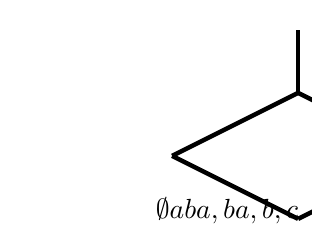
\begin{tikzpicture}[scale=0.8]
            \crd{0}{0}{$\emptyset$}
            \crd[above]{-2}{1}{$\s{a}$}
            \crd[above]{2}{1}{$\s{b}$}
            \crd[left]{0}{2}{$\s{a,b}$}
            \crd[left]{0}{3}{$\s{a,b,c}$}
            \draw [ultra thick] (0,0) -- (-2,1);
            \draw [ultra thick] (0,0) -- (2,1);
            \draw [ultra thick] (-2,1) -- (0,2);
            \draw [ultra thick] (2,1) -- (0,2);
            \draw [ultra thick] (0,2) -- (0,3);
        \end{tikzpicture} 
        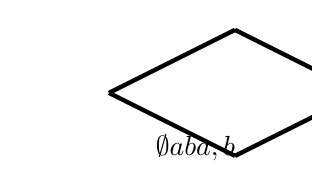
\begin{tikzpicture}[scale=0.8]
            \crd{0}{0}{$\emptyset$}
            \crd[above]{-2}{1}{$\s{a}$}
            \crd[above]{2}{1}{$\s{b}$}
            \crd[left]{0}{2}{$\s{a,b}$}
            \draw [ultra thick] (0,0) -- (-2,1);
            \draw [ultra thick] (0,0) -- (2,1);
            \draw [ultra thick] (-2,1) -- (0,2);
            \draw [ultra thick] (2,1) -- (0,2);
        \end{tikzpicture} 
    \end{center}
\end{frame}


\end{document}